\begin{savequote}[45mm]
\ascii{Any fool can write code that a computer can understand. Good programmers write code that humans can understand.}
\qauthor{\ascii{- Martin Flower}}
\end{savequote}

\chapter{本地执行} 
\label{ch:local}

\begin{content}

\tf{}可以独立地运行在一个进程内,完成计算图的执行过程。本章将重点介绍本地运行时的基本架构与运行机制;重点讨论计算图剪枝、分裂、优化、执行等实现技术细节;并且详细探究在本地模式下,跨设备间\ascii{OP}之间数据交互的工作机制,及其\ascii{OP}在设备上的编排(\ascii{placement})算法。

\end{content}

\section{本地模式}

\begin{content}

如\refig{local}所示,在本地模式下,\ascii{Client, Master, Worker}部署在同一台机器上,并运行在单独的进程内,各服务实体之间是函数调用关系。

\begin{figure}[H]
\centering
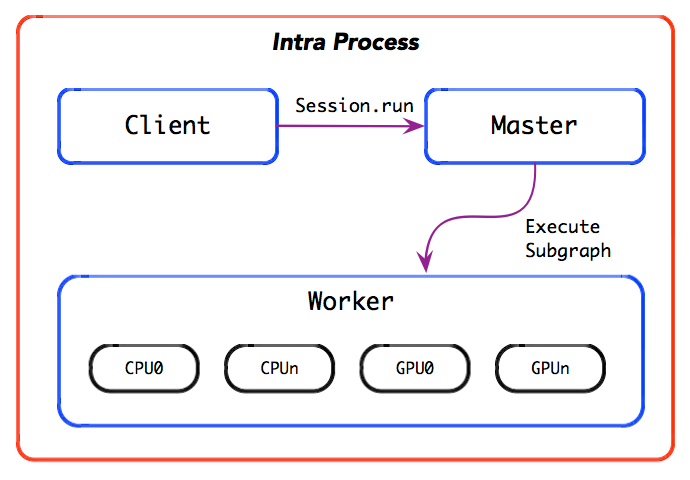
\includegraphics[width=0.7\textwidth]{figures/local.png}
\caption{本地模式}
 \label{fig:local}
\end{figure}

\subsection{运行时}

\ascii{Client}负责计算图的构造,通过调用\code{Session.run},启动计算图的执行过程。\ascii{Master}收到计算图执行命令后,启动计算图的剪枝操作,接着按照当前设备集完成图的分离,生成了很多子图;然后\ascii{Master}将子图注册给各个\ascii{Worker},触发各个\ascii{Worker}执行子图;每个\ascii{Worker}收到执行子图的命令后,将启动一个\ascii{Executor},按照子图的拓扑排序完成子图的执行。

\subsection{架构模型}

\begin{figure}[H]
\centering
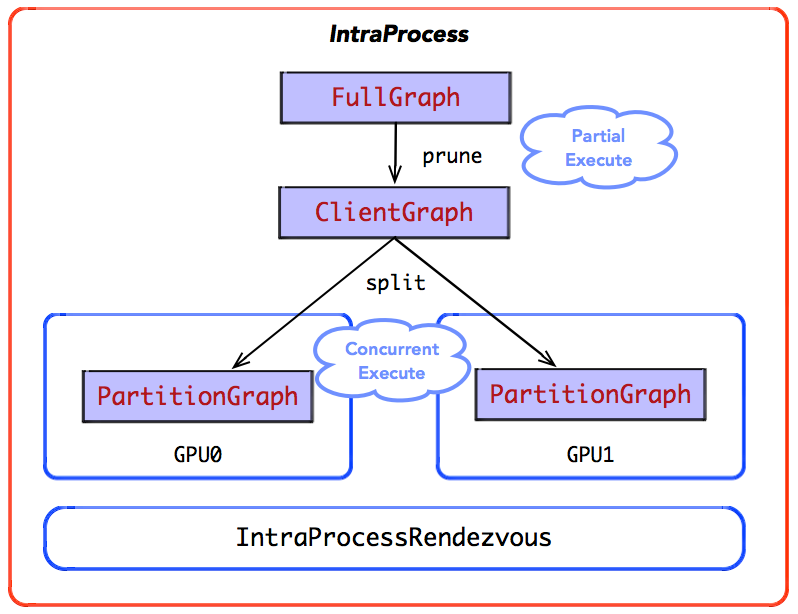
\includegraphics[width=0.8\textwidth]{figures/local-runtime.png}
\caption{本地运行时}
 \label{fig:local-runtime}
\end{figure}

\subsection{形式化}

在真实的系统实现中,本地运行时是使用\ascii{C++}实现,但涉及过多的实现细节,不易发现算法的主干和逻辑。为了简化问题的描述,将形式化地描述一次迭代执行的实现过程。

\begin{leftbar}
\begin{python}
def send_inputs(rendezvous, inputs):
  for input in inputs:
    rendezvous.send(input.key, input.tensor)

def recv_outputs(rendezvous, outputs):
  for output in outputs:
    rendezvous.recv(output.key, output.tensor)

def exec_partitions(executors_and_partitions):
  barrier = ExecutorBarrier(executors_and_partitions.size())
  for (executor, partition) in executors_and_partitions:
    executor.run(partition, barrier)
  barrier.wait()

def run_step(devices, full_graph, inputs, outputs):
  rendezvous = IntraProcessRendezvous(devices)
  send_intpus(rendezvous, inputs)
  client_graph = prune(full_graph, inputs, outputs)
  exec_partitions(split(client_graph, devices))
  recv_outputs(rendezvous, outputs)
\end{python}
\end{leftbar}

其中,在每个计算设备上,启动一个\code{Executor}执行分配给它的\code{PartitionGraph}。当某一个计算设备执行完所分配的\code{PartitionGraph}之后,\code{ExecutorBarrier}的计数器加\ascii{1},直至所有设备完成\code{PartitionGraph}列表的执行,\code{barrier.wait()}阻塞操作退出。

跨设备的\code{PartitionGraph}之间可能存在数据依赖关系,它们之间通过插入\code{Send/Recv}节点完成交互。事实上,在本地模式中,\code{Send/Recv}通过\code{Rendezvous}完成数据交换的。\code{Send}将数据放在\code{Rendezvous}上,而\code{Recv}则根据标识从\code{Rendezvous}取走。其中,\code{Send}不阻塞,而\code{Recv}是阻塞的。

因此,在\code{PartitionGraph}列表开始执行之前,需要先将\code{inputs}放置在\code{IntraProcessRendezvous}上;当\code{PartitionGraph}列表完成计算后,\code{outputs}将自动地从\code{IntraProcessRendezvous}上取走数据。

\section{会话控制}

在本地模式下,计算图执行的运行时由\code{DirectSession}控制。一般地,\code{DirectSession}执行计算图时,各组件之间都是函数调用关系。但是,\code{DirectSession}也存在清晰的生命周期管理机制,如\refig{local-direct-session-lifecycle}所示。

\begin{figure}[H]
\centering
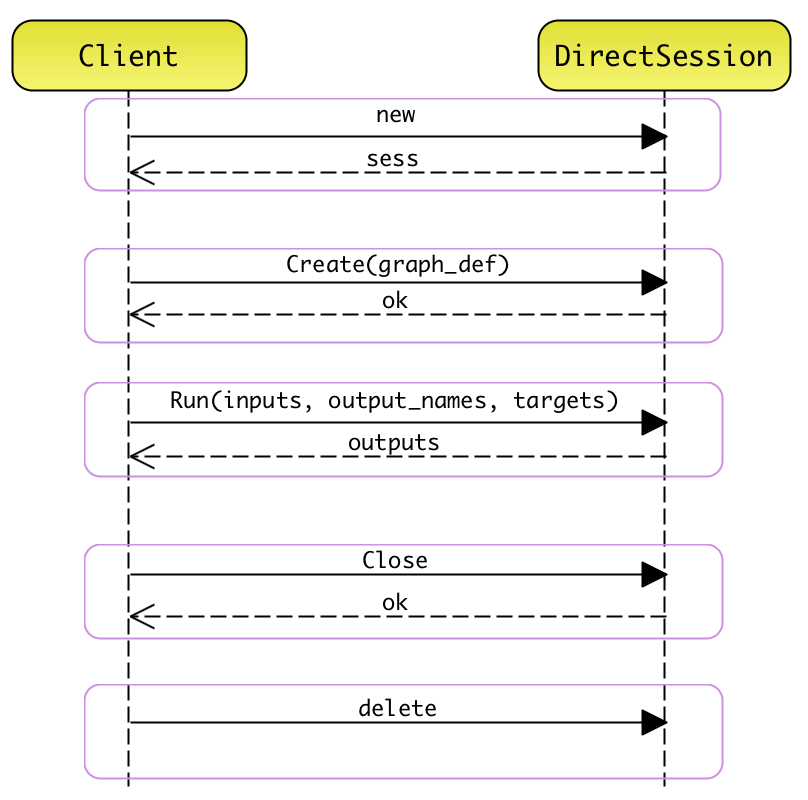
\includegraphics[width=0.6\textwidth]{figures/local-direct-session-lifecycle.png}
\caption{DirectSession生命周期}
 \label{fig:local-direct-session-lifecycle}
\end{figure}

\subsection{创建会话}

如\refig{local-direct-session-factory}所示,\code{DirectSession}由\code{DirectSessionFactory}多态创建。其中,\code{DeviceFactory::AddDevices}将创建本地设备集。

\begin{figure}[H]
\centering
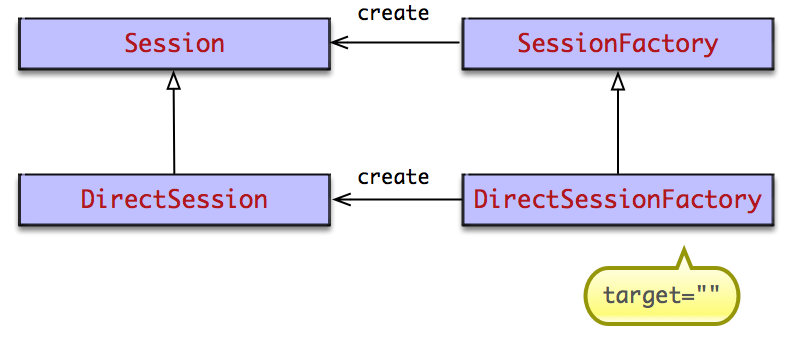
\includegraphics[width=0.6\textwidth]{figures/local-direct-session-factory.png}
\caption{多态创建DirectSession}
 \label{fig:local-direct-session-factory}
\end{figure}

\begin{leftbar}
\begin{c++}
struct DirectSessionFactory : SessionFactory {
  bool AcceptsOptions(const SessionOptions& options) override {
    return options.target.empty();
  }

  Session* NewSession(const SessionOptions& options) override {
    std::vector<Device*> devices;
    DeviceFactory::AddDevices(
        options, "/job:localhost/replica:0/task:0", &devices);
    return new DirectSession(options, new DeviceMgr(devices));
  }
};
\end{c++}
\end{leftbar}

\subsection{创建/扩展图}



\subsection{执行图}

\code{DirectSession::Run}是\tf{}运行时最重要的逻辑,它完成了一次迭代计算。

\subsection{关闭会话}

\begin{leftbar}
\begin{c++}
Status DirectSession::Close() {
  cancellation_manager_->StartCancel();
  {
    mutex_lock l(closed_lock_);
    if (closed_) return Status::OK();
    closed_ = true;
  }
  return Status::OK();
}
\end{c++}
\end{leftbar}

如\refig{local-cancellation-manager}所示,将\ascii{Step}注册给\code{DirectSession}的\code{CancellationManager}之中。当\code{DirectSession}被关闭时,\code{DirectSession}的\code{CancellationManager},将取消这次\ascii{step}的执行过程。

\begin{figure}[H]
\centering
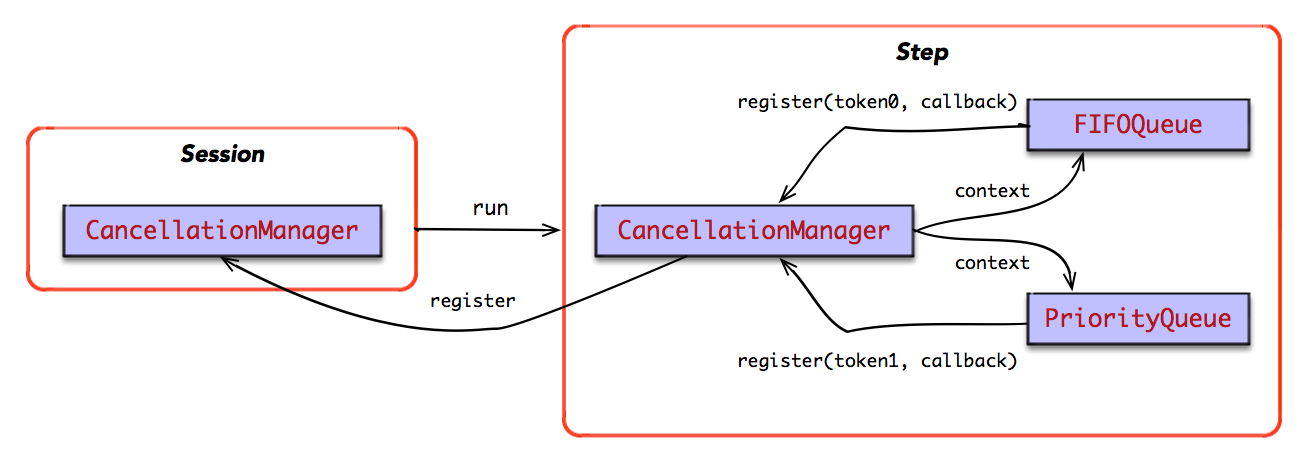
\includegraphics[width=0.9\textwidth]{figures/local-cancellation-manager.png}
\caption{CancellationManager工作原理}
 \label{fig:local-cancellation-manager}
\end{figure}

\begin{leftbar}
\begin{c++}
Status DirectSession::Run(
   const NamedTensorList& inputs,
   const std::vector<string>& output_names,
   const std::vector<string>& target_nodes,
   std::vector<Tensor>* outputs) {
  // step\_cancellation\_manager is passed to `OpKernelContext`
  CancellationManager step_cancellation_manager;

  // Register this step with session's cancellation manager, so that
  // `Session::Close()` will cancel the step.
  CancellationToken cancellation_token =
      cancellation_manager_->get_cancellation_token();
  bool already_cancelled = !cancellation_manager_->RegisterCallback(
      cancellation_token, [&step_cancellation_manager]() {
        step_cancellation_manager.StartCancel();
      });
  // ignore others...
}
\end{c++}
\end{leftbar}

当前\ascii{Step}的\code{CancellationManager}最终会传递给\code{OpKernelContext}。\ascii{Kernel}实现计算时,如果保存了中间状态,可以向其注册相应的回调钩子。其中,每个回调钩子都有唯一的\code{token}标识。

当\ascii{Step}被取消时,回调钩子被调用,该\ascii{Kernel}可以取消该\ascii{OP}的计算。例如,\code{FIFOQueue}实现\code{TryEnqueue}时,便往本次\ascii{Step}的\code{CancellationManager}注册了回调钩子,用于取消该\ascii{Kernel}中间的状态信息。

\begin{leftbar}
\begin{c++}
void FIFOQueue::TryEnqueue(const Tuple& tuple, OpKernelContext* ctx,
                           DoneCallback callback) {
  CancellationManager* cm = ctx->cancellation_manager();
  CancellationToken token = cm->get_cancellation_token();
  bool already_cancelled;
  {
    mutex_lock l(mu_);
    already_cancelled = !cm->RegisterCallback(
        token, [this, cm, token]() { Cancel(kEnqueue, cm, token); });
  }
  // ignore others...
}
\end{c++}
\end{leftbar}

\section{图操作}

如\refig{local-graph-transformation}所示,在本地模式下,计算图经历三个形态的变换,最终被分解至各个计算设备上,以便实现在各个计算设备上并发执行子图。

\begin{figure}[H]
\centering
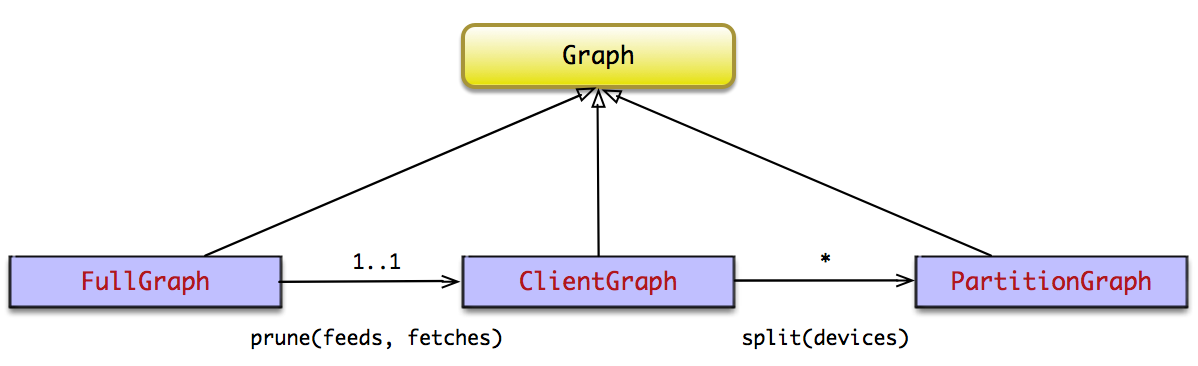
\includegraphics[width=0.9\textwidth]{figures/local-graph-transformation.png}
\caption{图变换}
 \label{fig:local-graph-transformation}
\end{figure}

\begin{itemize}
  \item \code{FullGraph}: \ascii{Client}负责构造的完整的计算图,常称为\code{FullGraph};但是,一次\code{Session.run}并不会执行整个计算图;
  \item \code{ClientGraph}: \ascii{Master}根据\code{Session.run}传递\code{feeds, fetches}输入输出列表,对\ascii{FullGraph}实施剪枝操作,计算得到本地迭代执行的最小依赖子图,常称为\code{ClientGraph};
  \item \code{PartitionGraph}: \ascii{Master}根据当前计算设备集,及其\ascii{OP}的设备约束规范,将\code{ClientGraph}分裂为多个\code{PartitionGraph};其中,每个计算设备对应一个\code{PartitionGraph},计算设备负责\code{PartitionGraph}的执行。
\end{itemize}

但是,\code{FullGraph, ClientGraph, PartitionGraph}的数据结构相同,它们都是\code{Graph}三种不同表现形式,仅仅大小和范畴存在差异。

\subsection{剪枝}

\subsection{分裂}

\subsection{优化}

\subsection{执行}

\section{OP编排}
